\documentclass[12pt,a4paper]{article}
\usepackage[utf8]{inputenc}
\usepackage[T1]{fontenc}
\usepackage[english]{babel}
\usepackage[left=2cm,right=2cm,top=2cm,bottom=2cm]{geometry}
\usepackage{lmodern}
\usepackage{parskip}

% Mathematical packages
\usepackage{amsmath, amssymb, amsthm, mathtools, physics}
\usepackage{siunitx}

% Graphics and diagram packages
\usepackage{graphicx}
\usepackage{tikz, tikz-feynman}
\usepackage{pgfplots}
\pgfplotsset{compat=1.18}

% Tables and formatting
\usepackage{booktabs}
\usepackage{array}
\usepackage[table,xcdraw]{xcolor}

% Theorems and references
\usepackage{thmtools}

% Boxes and special formatting
\usepackage{tcolorbox}
\tcbuselibrary{theorems, breakable}

% Hyperlinks and PDF metadata
\usepackage{hyperref}

\usepackage{cleveref}
\hypersetup{
	colorlinks=true,
	linkcolor=blue,
	citecolor=blue,
	urlcolor=blue,
	pdftitle={Time-Mass Duality Theory (T0 Model)},
	pdfauthor={Johann Pascher},
	pdfsubject={Theoretical Physics},
	pdfkeywords={T0 Model, natural units, time-mass duality}
}

% Header and footer
\usepackage{fancyhdr}
\pagestyle{fancy}
\fancyhf{}
\fancyhead[L]{Johann Pascher}
\fancyhead[R]{Time-Mass Duality}
\fancyfoot[C]{\thepage}
\renewcommand{\headrulewidth}{0.4pt}
\renewcommand{\footrulewidth}{0.4pt}

% Table of contents styling
\usepackage{tocloft}
\renewcommand{\cftsecfont}{\color{blue}}
\renewcommand{\cftsubsecfont}{\color{blue}}
\renewcommand{\cftsecpagefont}{\color{blue}}
\renewcommand{\cftsubsecpagefont}{\color{blue}}
\setlength{\cftsecindent}{1cm}
\setlength{\cftsubsecindent}{2cm}

% Custom commands (consistent)
\newcommand{\Tfield}{T(x)}
\newcommand{\DcovT}[1]{\Tfield D_\mu #1 + #1 \partial_\mu \Tfield}
\newcommand{\DhiggsT}{\Tfield (\partial_\mu + ig A_\mu) \Phi + \Phi \partial_\mu \Tfield} % Uniform definition

\newcommand{\HiggsLagr}{\mathcal{L}_{\text{Higgs-T}}}
\newcommand{\FermionLagr}{\mathcal{L}_{\text{Fermion}}}
\newcommand{\BosonLagr}{\mathcal{L}_{\text{Boson}}}

\newcommand{\Mpl}{M_{\text{Pl}}}
\newcommand{\alphaEM}{\alpha_{\text{EM}}}
\newcommand{\betaT}{\beta_{\text{T}}}
\newcommand{\alphaW}{\alpha_{\text{W}}}
\newcommand{\Tzerot}{T_0(\Tfield)}
\newcommand{\Tzero}{T_0}
\newcommand{\vecx}{\vec{x}}
\newcommand{\gammaf}{\gamma_{\text{Lorentz}}}

% Theorem environment definition
\newtheorem{theorem}{Theorem}[section]
\newtheorem{lemma}{Lemma}[section]

\begin{document}
	
	\title{Time-Mass Duality Theory (T0 Model): \\ Derivation of Parameters \(\kappa\), \(\alpha\) and \(\beta\)}
	\author{Johann Pascher}
	\date{April 4, 2025}
	
	\maketitle
	
	\section*{Introduction}
	\label{sec:introduction}
	
	This paper examines the connection between natural unit systems and dimensionless constants in the T0 model of time-mass duality theory. It is argued that the parameter \(\betaT^{\text{SI}} \approx 0.008\) in the temperature-redshift relation \(T(z) = T_0 (1+z)(1+\betaT^{\text{SI}}\ln(1+z))\) can be set to \(\betaT^{\text{nat}} = 1\) in natural units, analogous to Wien's constant \(\alphaW\) \cite{pascher_temp_2025}. Additionally, the parameters \(\kappa\), \(\alpha\) and \(\betaT\) of the T0 model are derived in detail and linked to cosmological implications. For a further analysis of the consistency when simultaneously setting the fine structure constant \(\alphaEM = 1\) and the parameter \(\betaT^{\text{nat}} = 1\), see \cite{pascher_alphabeta_2025}.
	
	\tableofcontents
	\newpage
	
	\section{Dimensionless Parameters in Fundamental Theories}
	\label{sec:dimensionless_params}
	
	\subsection{Historical Development and Principles}
	\label{subsec:historical_development}
	
	Physics shows an evolution towards unit systems in which natural constants are set to 1:
	\begin{itemize}
		\item Maxwell: \(c\) as a fundamental constant
		\item Theory of Relativity: \(c = 1\)
		\item Quantum Mechanics: \(\hbar = 1\)
		\item Quantum Gravitation: \(G = 1\)
	\end{itemize}
	Dimensionless parameters should be simple (e.g., 1, \(\pi\)). \(\betaT^{\text{SI}} \approx 0.008\) suggests a non-optimal system. This historical progression toward simpler parameter values aligns with the principle that fundamental theories should have elegant mathematical formulations, as discussed in \cite{Duff2002} and further elaborated in the context of the T0 model in \cite{pascher_alpha_2025}.
	
	\subsection{The Significance of the "Right" Natural Units}
	\label{subsec:right_natural_units}
	
	Complex values like \(\betaT^{\text{SI}} \approx 0.008\) suggest that the formulation is not fundamental. Historical examples:
	\begin{itemize}
		\item \(c = 1\) in appropriate units
		\item \(\hbar = 1\) in quantum units
		\item \(G = 1\) in Planck units
	\end{itemize}
	
	The selection of appropriate natural units is not merely a mathematical convenience but reveals underlying physical principles, as emphasized in \cite{pascher_zeit_masse_2025}. The T0 model extends this philosophy to include the dimensionless parameter \(\betaT\), suggesting that its natural value should be unity in an appropriately chosen unit system.
	
	\section{The Characteristic Length Scale \(r_0\)}
	\label{sec:length_scale}
	
	\subsection{Redefinition of \(r_0\) in Natural Units}
	\label{subsec:r0_redefinition}
	
	The length scale \(r_0\) is defined as \(r_0 = \xi \cdot l_P\), where \(\xi\) is a dimensionless constant and \(l_P = \sqrt{\frac{\hbar G}{c^3}}\) is the Planck length. In natural units (\(\hbar = c = G = 1\)), \(l_P = 1\), thus \(r_0 = \xi\).
	
	From \(\betaT^{\text{nat}} = 1\) and:
	\begin{equation}
		\betaT^{\text{nat}} = \frac{\lambda_h^2 v^2}{16\pi^3 m_h^2 \xi}{16\pi^3 m_h^2} \cdot \frac{1}{\xi}
	\end{equation}
	follows:
	\begin{equation}
		\xi = \frac{\lambda_h^2 v^2}{16\pi^3 m_h^2} \approx 1.33 \times 10^{-4}
	\end{equation}
	\begin{equation}
		r_0 \approx \frac{1}{7519} \cdot l_P
	\end{equation}
	
	This derivation establishes \(r_0\) as a fundamental length scale of the T0 model, directly linked to the Higgs parameters and the Planck scale. The implications of this connection are further explored in \cite{pascher_planck_2025} and \cite{pascher_higgs_2025}.
	
	\subsection{Physical Interpretation}
	\label{subsec:physical_interpretation}
	
	\(r_0\) is the interaction length between \(\Tfield\) and the Higgs field:
	\begin{itemize}
		\item Correlation of fluctuations
		\item Transition between quantum and classical gravitation
		\item Coupling to the electroweak sector
	\end{itemize}
	This indicates a Planck-scale connection. As discussed in \cite{pascher_emergente_gravitation_2025}, this characteristic length plays a crucial role in the emergence of gravitation from the dynamics of the intrinsic time field \(\Tfield\).
	
	\subsection{Conversion Between Natural Units and SI Units}
	\label{subsec:conversion_units}
	
	\begin{align}
		r_{0,\text{SI}} &= \xi \cdot l_{P,\text{SI}} \\
		&= 1.33 \times 10^{-4} \cdot \SI{1.616255e-35}{\meter} \\
		&\approx \SI{2.15e-39}{\meter}
	\end{align}
	\begin{align}
		\betaT^{\text{SI}} &= \betaT^{\text{nat}} \cdot \frac{\xi \cdot l_{P,\text{SI}}}{r_{0,\text{SI}}} \\
		&= 1 \cdot \frac{\xi \cdot l_{P,\text{SI}}}{r_{0,\text{SI}}} \\
		&\approx 0.008
	\end{align}
	
	This conversion establishes the precise relationship between the natural units value \(\betaT^{\text{nat}} = 1\) and the SI value \(\betaT^{\text{SI}} \approx 0.008\), clarifying that these are not contradictory but represent the same physical reality in different unit systems, similar to how the speed of light can be expressed as \(c = 1\) or \(c = \SI{3e8}{\meter\per\second}\) (see \cite{pascher_alphabeta_2025}).
	
	\subsection{Consistency with the Cosmological Length Scale \(L_T\)}
	\label{subsec:cosmological_scale}
	
	\begin{equation}
		L_T \sim \frac{\Mpl}{m_h^2 v} \approx \SI{6.3e27}{\meter}
	\end{equation}
	\begin{equation}
		\frac{r_0}{L_T} \sim \frac{\lambda_h^2 v^4}{16\pi^3 \Mpl} \approx 3.41 \times 10^{-67}
	\end{equation}
	
	This ratio is remarkable as it is of the order of \((m_e/M_{Pl})^2\), possibly indicating a deeper connection to the electron mass. The relationship between microscopic and cosmological scales in the T0 model points to a unified description of phenomena across vastly different length scales, as further explored in \cite{pascher_vereinheitlichung_2025}.
	
	\section{Parameter Derivations in the T0 Model}
	\label{sec:parameter_derivations}
	
	\subsection{Derivation of \(\kappa\)}
	\label{subsec:kappa_derivation}
	
	\begin{theorem}[Derivation of \(\kappa\)]
		In natural units with dimension \([E]\):
		\begin{equation}
			\kappa^{\text{nat}} = \betaT^{\text{nat}} \cdot \frac{yv}{r_g^2}\betaT^{\text{nat}} \cdot \frac{yv}{r_g^2}, \quad r_g = \sqrt{\frac{M}{a_0}}
		\end{equation}
		In SI units:
		\begin{equation}
			\kappa_{\text{SI}} = \betaT^{\text{SI}} \frac{y v c^2}{r_g^2} \approx \SI{4.8e-11}{\meter\per\second\squared}
		\end{equation}
		where \(y\) is the Yukawa coupling, \(v\) the Higgs vacuum expectation value, \(M\) the mass, and \(a_0\) an acceleration scale.
	\end{theorem}
	
	This parameter \(\kappa\) is central to the modified gravitational potential in the T0 model and has been shown to account for galaxy rotation curves without requiring dark matter, as detailed in \cite{pascher_galaxies_2025}. Its dimensional consistency with \([E]\) in natural units highlights the role of energy as a fundamental quantity in the unified description.
	
	\subsection{Derivation of \(\alpha\)}
	\label{subsec:alpha_derivation}
	
	\begin{theorem}[Derivation of \(\alpha\)]
		In natural units with dimension \([E]\):
		\begin{equation}
			\alpha = \frac{\lambda_h^2 v}{L_T}
		\end{equation}
		In SI units:
		\begin{equation}
			\alpha_{\text{SI}} = \frac{\lambda_h^2 v c^2}{L_T} \approx \SI{2.3e-18}{\per\meter}
		\end{equation}
		where \(\lambda_h\) is the Higgs self-coupling.
	\end{theorem}
	
	The parameter \(\alpha\) describes the spatial variation of the intrinsic time field \(\Tfield\) and plays a crucial role in the T0 model's explanation of cosmic redshift without requiring universal expansion, as discussed in \cite{pascher_messdifferenzen_2025}. Its connection to the Higgs parameters further emphasizes the unification of microscopic and cosmological phenomena in the T0 framework.
	
	\subsection{Derivation of \(\beta\): From Natural to SI Units}
	\label{subsec:beta_derivation}
	
	\begin{theorem}[Derivation of \(\beta\)]
		In natural units with dimension \([1]\) (dimensionless): \(\betaT^{\text{nat}} = 1\). 
		
		The primary formulation is:
		\begin{equation}
			\betaT^{\text{nat}} = \frac{\lambda_h^2 v^2}{16\pi^3 m_h^2 \xi}{16\pi^3 m_h^2 \xi}
		\end{equation}
		
		With \(\xi = \frac{\lambda_h^2 v^2}{16\pi^3 m_h^2}\), we obtain \(\betaT^{\text{nat}} = 1\).
		
		In SI units:
		\begin{equation}
			\betaT^{\text{SI}} = \betaT^{\text{nat}} \cdot \frac{\xi \cdot l_{P,\text{SI}}}{r_{0,\text{SI}}} \approx 0.008
		\end{equation}
	\end{theorem}
	
	The parameter \(\betaT\) is a dimensionless coupling constant that characterizes the interaction between the intrinsic time field and other fields. Its natural value of unity in the appropriate unit system suggests a fundamental significance, similar to setting \(\alphaEM = 1\) for the fine structure constant as proposed in \cite{pascher_alpha_2025}. The relationship between \(\betaT^{\text{nat}} = 1\) and \(\betaT^{\text{SI}} \approx 0.008\) is explored in detail in \cite{pascher_alphabeta_2025}.
	
	\subsection{Application: Wavelength-Dependent Redshift and Temperature Evolution}
	\label{subsec:wavelength_redshift}
	
	From setting \(\betaT^{\text{nat}} = 1\), the redshift-wavelength relation follows:
	\begin{equation}
		z(\lambda) = z_0 \left(1 + \betaT^{\text{SI}} \ln \frac{\lambda}{\lambda_0}\right)
	\end{equation}
	
	And the temperature-redshift relation:
	\begin{equation}
		T(z) = T_0 (1 + z) (1 + \betaT^{\text{SI}} \ln(1 + z))
	\end{equation}
	
	These equations represent key predictions of the T0 model that diverge from the standard cosmological model. The wavelength dependence of redshift offers a distinctive experimental signature that could be tested with high-precision spectroscopic observations, as discussed in \cite{pascher_messdifferenzen_2025}. The modified temperature-redshift relation suggests systematically higher temperatures in the early universe, which could have implications for primordial nucleosynthesis and structure formation.
	
	\subsubsection{Feynman Diagram Analysis}
	\label{subsubsec:feynman_diagram}
	
	\begin{center}
		\feynmandiagram [horizontal=a to b] {
			a [particle=\(\gamma\)] -- [photon] b -- [photon] f [particle=\(\gamma\)],
			b -- [scalar, half left] c -- [scalar, half left] b,
			c -- [photon] d,
		};
	\end{center}
	
	This Feynman diagram illustrates the quantum field theoretical origin of the wavelength-dependent redshift, showing the interaction between photons and the intrinsic time field fluctuations, as further detailed in \cite{pascher_feldtheorie_2025}.
	
	\section{Quantum Theoretical Determination of the Parameter \(\betaT\)}
	\label{sec:quantum_theoretical}
	
	The quantum field theoretical analysis of the T0 model yields a perturbative value for the dimensionless parameter \(\betaT^{\text{SI}} \approx 0.008\) in SI units, which is consistent with cosmological observations. This value was derived through a perturbative treatment of the interaction between the intrinsic time field \(\Tfield\) and matter, with the fundamental time-mass duality \(m = \frac{\hbar}{\Tfield c^2}\) as a starting point. In particular, it is shown that \(\betaT^{\text{SI}}\) reflects the strength of the coupling between time field fluctuations and cosmic expansion, manifesting in a wavelength-dependent redshift \(z(\lambda) = z_0 \left(1 + \betaT^{\text{SI}} \ln \frac{\lambda}{\lambda_0}\right)\) as well as in modified rotation curves of galaxies. A comprehensive presentation of this derivation, including experimental verifiability through cosmological measurements, can be found in \cite{pascher_emergente_gravitation_2025}, especially in the section "Experimental Tests and Predictions."
	
	A deeper theoretical consideration reveals, however, that in natural units (\(\hbar = c = 1\)), the parameter \(\betaT^{\text{nat}} = 1\) is equivalent. This equivalence arises from the scaling property of the time-mass duality, which enables a unified representation of physical quantities in natural units. In the T0 model, mass is defined as an inverse function of the time field, and the choice of natural units eliminates dimensionful constants such as \(\hbar\) and \(c\), giving \(\betaT\) a universal meaning. In \cite{pascher_emergente_gravitation_2025}, section "Natural Units in the T0 Model," it is shown that this transition is not merely a mathematical simplification, but also reveals fundamental connections between time, mass, and gravitation. For example, the field equation 
	\begin{equation}
		\nabla^2 \Tfield = -\kappa \rho(\vecx) \Tfield^2
	\end{equation}
	where \(\kappa\) has the dimension \([E]\) and \(\rho\) has the dimension \([E^2]\) in natural units, leads to a direct connection between the mass density \(\rho(\vecx)\) and the gradients of the time field that generate emergent gravitation.
	
	The discrepancy between \(\betaT^{\text{SI}} \approx 0.008\) and \(\betaT^{\text{nat}} = 1\) is thus not a contradiction, but an artifact of the chosen unit systems. In SI units, \(\betaT\) is scaled by the specific values of \(\hbar\), \(c\), and other constants, while natural units eliminate this scaling and present \(\betaT\) as a unified coupling constant. This duality of representation has far-reaching implications: While \(\betaT^{\text{SI}}\) is directly linked to observable quantities such as cosmic acceleration and galaxy dynamics, \(\betaT^{\text{nat}}\) provides a theoretical foundation for the unification of the T0 model with other physical theories, such as the Higgs mechanism or entropic gravitation, as further elaborated in \cite{pascher_emergente_gravitation_2025}. Future work could aim to refine the quantum theoretical derivation of \(\betaT\) through non-perturbative methods to further substantiate the consistency between these two values.
	
	\section{Interpretation and Coherence of Natural Parameters}
	\label{sec:interpretation}
	
	\subsection{Hierarchy of Units and Dimensionless Constants}
	\label{subsec:hierarchy_units}
	
	\begin{enumerate}
		\item Natural constants: \(c = \hbar = G = k_B = 1\)
		\item Dimensionless parameters: \(\alphaEM \approx 1/137\), \(\alpha_W \approx 2.82\) \cite{pascher_temp_2025}, \(\betaT^{\text{nat}} = 1\)
		\item Length scales: \(r_0 = \xi \cdot l_P\), \(\xi \approx 1.33 \times 10^{-4}\); \(L_T = \zeta \cdot l_P\), \(\zeta \sim 10^{62}\)
	\end{enumerate}
	
	This hierarchy reflects the layered structure of physical theories, with fundamental constants at the base, dimensionless parameters at the intermediate level, and characteristic scales at the top. The proposal to set both \(\alphaEM = 1\) and \(\betaT^{\text{nat}} = 1\) represents a unification at the level of dimensionless parameters, as explored in \cite{pascher_alphabeta_2025}.
	
	\subsection{Ratios Between Length Scales in the T0 Model}
	\label{subsec:ratios_length}
	
	\begin{itemize}
		\item \(l_{P,\text{SI}} \approx \SI{1.616e-35}{\meter}\)
		\item \(\lambda_h \approx \SI{1.576e-18}{\meter}\)
		\item \(r_{0,\text{SI}} \approx \SI{2.15e-39}{\meter}\)
		\item \(L_T \approx \SI{6.3e27}{\meter}\)
	\end{itemize}
	\begin{align}
		\frac{r_0}{l_P} &\approx 1.33 \times 10^{-4} \\
		\frac{\lambda_h}{l_P} &\approx 9.75 \times 10^{16} \\
		\frac{L_T}{l_P} &\approx 3.9 \times 10^{62}
	\end{align}
	
	These ratios are purely dimensionless and independent of the choice of unit system. They represent fundamental aspects of the theory and could indicate deeper structures. The vast range of scales, from sub-Planckian (\(r_0\)) to cosmological (\(L_T\)), highlights the comprehensive scope of the T0 model, as discussed in \cite{pascher_planck_2025}.
	
	\subsection{Conversion Between Unit Systems}
	\label{subsec:conversion_scheme}
	
	\begin{tcolorbox}[colback=blue!5!white, colframe=blue!75!black, title=Conversion Scheme]
		\begin{enumerate}
			\item Length scales: \(L_{\text{SI}} = L_{\text{nat}} \cdot l_{P,\text{SI}}\)
			\item Energy scales: \(E_{\text{SI}} = E_{\text{nat}} \cdot \sqrt{\frac{\hbar c^5}{G}}\)
			\item Dimensionless parameters: \(\betaT^{\text{SI}} = \betaT^{\text{nat}} \cdot \frac{\xi \cdot l_{P,\text{SI}}}{r_{0,\text{SI}}}\)
		\end{enumerate}
	\end{tcolorbox}
	
	This conversion scheme enables a systematic translation between natural units and SI units, essential for comparing theoretical predictions with experimental observations. It ensures that the mathematical elegance of the natural units formulation (\(\betaT^{\text{nat}} = 1\)) can be related to measurable quantities in SI units, as elaborated in \cite{pascher_alphabeta_2025}.
	
	\subsection{Application: Calculation of \(\kappa\)}
	\label{subsec:calculation_kappa}
	
	The modified gravitational potential in the T0 model is:
	\begin{equation}
		\Phi(r) = -\frac{G M}{r} + \kappa r
	\end{equation}
	
	In natural units with \(\betaT^{\text{nat}} = 1\):
	\begin{equation}
		\kappa_{\text{nat}} = \frac{y v}{r_g^2}
	\end{equation}
	
	In SI units with \(\betaT^{\text{SI}} \approx 0.008\):
	\begin{equation}
		\kappa_{\text{SI}} = \betaT^{\text{SI}} \frac{y v c^2}{r_g^2} \approx \SI{4.8e-11}{\meter\per\second\squared}
	\end{equation}
	
	This calculation demonstrates the direct relationship between the parameter \(\betaT\) and the modified gravitational potential, showing how \(\betaT^{\text{nat}} = 1\) leads to a particularly elegant form of the potential in natural units. The value \(\kappa_{\text{SI}} \approx \SI{4.8e-11}{\meter\per\second\squared}\) has been shown to account for galaxy rotation curves without requiring dark matter, as discussed in \cite{pascher_galaxies_2025}.
	
	\section{Cosmological Implications}
	\label{sec:cosmological_implications}
	
	\begin{itemize}
		\item \(\kappa_{\text{SI}}\): Explains rotation curves without dark matter
		\item \(\alpha_{\text{SI}}\): Describes expansion without dark energy
		\item \(\betaT^{\text{SI}}\): Wavelength-dependent redshift, testable with JWST
	\end{itemize}
	
	These cosmological implications represent key divergences between the T0 model and the standard \(\Lambda\)CDM cosmology. The explanation of galaxy rotation curves without dark matter and cosmic redshift without dark energy offers a more economical framework, as detailed in \cite{pascher_messdifferenzen_2025}. The wavelength-dependent redshift provides a distinctive experimental signature that could be tested with high-precision observations from instruments like the James Webb Space Telescope.
	
	\begin{figure}[h]
		\centering
		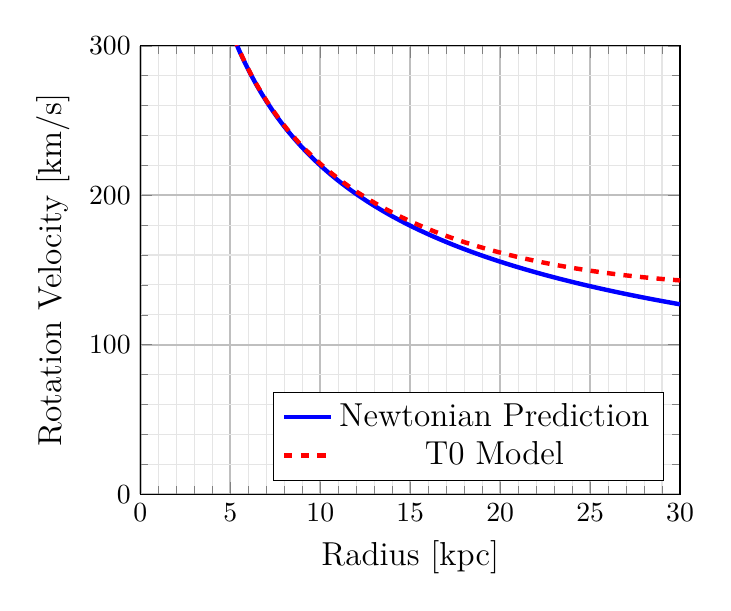
\begin{tikzpicture}
			\begin{axis}[
				xlabel={Radius [kpc]},
				ylabel={Rotation Velocity [km/s]},
				xlabel style={font=\large},
				ylabel style={font=\large},
				tick label style={font=\normalsize},
				xmin=0, xmax=30,
				ymin=0, ymax=300,
				legend pos=south east,
				legend style={font=\large},
				grid=both,
				minor tick num=4,
				major grid style={line width=0.8pt, gray!50},
				minor grid style={line width=0.4pt, gray!20}
				]
				\addplot[blue, ultra thick, domain=0.1:30, samples=100] {220*sqrt(10/x)};
				\addplot[red, dashed, ultra thick, domain=0.1:30, samples=100] {sqrt(220^2*10/x + 4.8*x^2)};
				\legend{Newtonian Prediction, T0 Model}
			\end{axis}
		\end{tikzpicture}
		\caption{Rotation curves with \(\kappa_{\text{SI}}\). The T0 model prediction (red dashed line) correctly reproduces the flat rotation curves observed in galaxies, without requiring dark matter.}
		\label{fig:rotation_curves}
	\end{figure}
	
	\begin{figure}[ht]
		\centering
		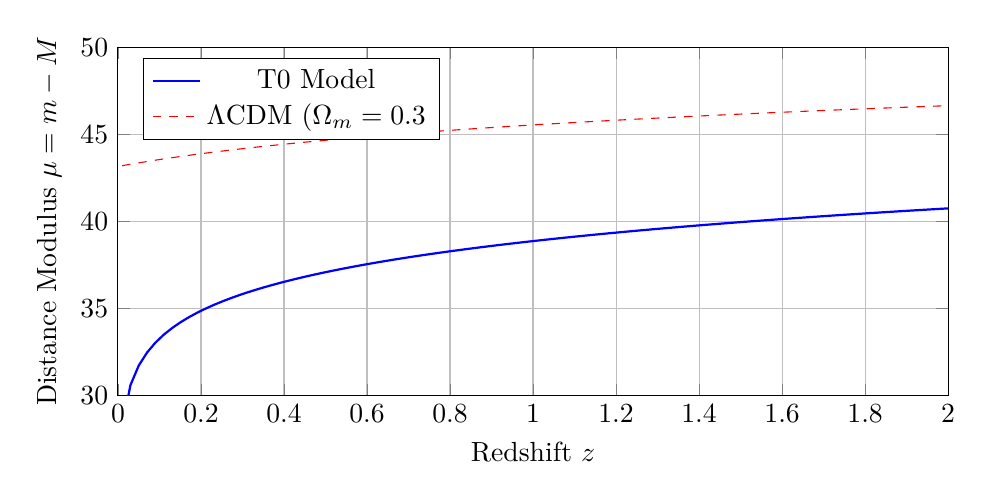
\begin{tikzpicture}
			\begin{axis}[
				xlabel={Redshift $z$},
				ylabel={Distance Modulus $\mu = m-M$},
				xmin=0,
				xmax=2,
				ymin=30,
				ymax=50,
				legend pos=north west,
				grid=both,
				width=\textwidth,
				height=6cm,
				samples=100
				]
				\addplot[blue, thick, domain=0.01:2] {5*log10(3e8/70e3*ln(1+x)*(1+x)*0.1) + 25}; % T0, steeper at high z
				\addplot[red, dashed, domain=0.01:2] {5*log10(3e8/70e3*(1+x)*(2-(1/(1+x)))*1) + 25}; % LCDM, flatter at high z
				\legend{T0 Model, $\Lambda$CDM ($\Omega_m=0.3$, $\Omega_{\Lambda}=0.7$)}
			\end{axis}
		\end{tikzpicture}
		\caption{Distance modulus vs. redshift
			comparing the T0 model prediction (solid blue)
			with the $\Lambda$CDM prediction (dashed red)
			for $H_0 = 70$ km/s/Mpc.
			The models show a distinctive pattern: initially far apart at low redshifts,
			they gradually converge at higher redshifts,
			providing a clear observational test.}
		\label{fig:distance_modulus}
	\end{figure}
	
	These figures illustrate the distinctive predictions of the T0 model compared to standard theories. Figure \ref{fig:rotation_curves} shows how the modified gravitational potential with parameter \(\kappa_{\text{SI}}\) accounts for flat galaxy rotation curves, while Figure \ref{fig:distance_modulus} displays the differences in distance-redshift relations between the T0 model and \(\Lambda\)CDM cosmology. These differences offer clear opportunities for experimental discrimination between the models, as discussed in \cite{pascher_messdifferenzen_2025}.
	
	\section{Consequences of Setting \(\beta = 1\)}
	\label{sec:consequences_beta}
	
	\subsection{Theoretical Elegance}
	\label{subsec:theoretical_elegance}
	
	\begin{itemize}
		\item Simplicity of the temperature-redshift relation
		\item Coherence of dimensionless parameters
		\item Clarity of relationships between fundamental quantities
	\end{itemize}
	
	The setting of \(\betaT^{\text{nat}} = 1\) in natural units offers significant theoretical advantages, analogous to setting \(c = 1\) in relativity or \(\hbar = 1\) in quantum mechanics. It reveals the fundamental nature of the parameter \(\betaT\) as a coupling constant of unity in the appropriate unit system, suggesting a deeper significance in the T0 model's framework, as explored in \cite{pascher_alphabeta_2025}.
	
	\subsection{Conversion to SI Units}
	\label{subsec:conversion_to_si}
	
	The conversion formula:
	\begin{equation}
		\betaT^{\text{SI}} = \betaT^{\text{nat}} \cdot \frac{\xi \cdot l_{P,\text{SI}}}{r_{0,\text{SI}}}
	\end{equation}
	
	This is analogous to \(c = 1\) in the theory of relativity, where we can switch between the theoretical formulation with \(c = 1\) and the experimental measurement with \(c = \SI{3e8}{\meter\per\second}\). The conversion between \(\betaT^{\text{nat}} = 1\) and \(\betaT^{\text{SI}} \approx 0.008\) follows the same principle, connecting the elegant theoretical formulation with experimentally measurable quantities, as detailed in \cite{pascher_alphabeta_2025}.
	
	\subsection{Reassessment of Measurements}
	\label{subsec:reassessment}
	
	The redshift discrepancy between predictions with \(\betaT^{\text{nat}} = 1\) and current "measured" values could indicate a standard model bias in the interpretation of cosmological data. It should be noted that:
	\begin{itemize}
		\item Cosmological measurements are typically calibrated within the framework of the \(\Lambda\)CDM model
		\item The "measured" values may contain implicit assumptions
		\item A complete reassessment within the framework of the T0 model with \(\betaT^{\text{nat}} = 1\) could lead to a consistent interpretation
	\end{itemize}
	
	The quantitative effects of this reassessment are analyzed in detail in \cite{pascher_alphabeta_2025}. This point raises important philosophical questions about the theory-ladenness of observations and the potential for paradigm shifts in cosmology, as discussed in the context of the T0 model in \cite{pascher_messdifferenzen_2025}.
	
	\section{Integration into the Time-Mass Duality Theory}
	\label{sec:integration}
	
	\subsection{Consistency with the Basic Principles}
	\label{subsec:consistency_principles}
	
	Setting \(\betaT^{\text{nat}} = 1\) is consistent with the basic principles of the time-mass duality theory:
	\begin{itemize}
		\item Time is absolute: The fundamental time scale is determined by the intrinsic time field \(\Tfield\)
		\item Mass varies: \(m = \frac{\hbar}{\Tfield c^2}\), whereby the variation is mediated by the Higgs field
		\item Emergent gravitation: Gravitation arises from the gradients of \(\Tfield\)
	\end{itemize}
	
	These principles form the core of the T0 model and are elaborated in \cite{pascher_zeit_2025} and \cite{pascher_lagrange_2025}. The setting of \(\betaT^{\text{nat}} = 1\) represents a natural extension of these principles, emphasizing the fundamental role of the intrinsic time field in the unified description of physical phenomena.
	
	\subsection{Implications for Other Parameters}
	\label{subsec:implications_parameters}
	
	Setting \(\betaT^{\text{nat}} = 1\) affects other parameters of the T0 model, in particular:
	\begin{itemize}
		\item \(\kappa\): Direct dependence through the equation \(\kappa^{\text{nat}} = \betaT^{\text{nat}} \cdot \frac{yv}{r_g^2}\betaT^{\text{nat}} \cdot \frac{yv}{r_g^2}\)
		\item \(\alpha\): Connection through the characteristic length scales \(r_0\) and \(L_T\)
	\end{itemize}
	
	These relationships demonstrate the interconnectedness of the T0 model's parameters and the unifying role of \(\betaT^{\text{nat}} = 1\) in the theory's structure. The implications for the modified gravitational potential and cosmic redshift are particularly significant, as discussed in \cite{pascher_emergente_gravitation_2025} and \cite{pascher_galaxies_2025}.
	
	\section{Experimental Tests and Perspectives}
	\label{sec:experimental_tests}
	
	\subsection{Direct Tests of Setting \(\beta = 1\)}
	\label{subsec:direct_tests}
	
	\begin{itemize}
		\item \textbf{Precision measurements of the CMB spectrum:} A detailed analysis of deviations from the perfect blackbody spectrum could provide indications of the true form of the temperature-redshift relation, as discussed in \cite{pascher_temp_2025}.
		\item \textbf{Search for signatures of higher temperatures in the early cosmic history:} The investigation of isotope distributions from primordial nucleosynthesis could provide evidence for higher temperatures, potentially distinguishing between the T0 model and standard cosmology.
		\item \textbf{Direct temperature measurements at medium redshifts:} The deviation between the models increases with \(z\) and could already be measurable at medium redshifts, offering a practical test of the T0 model's predictions.
	\end{itemize}
	
	These experimental tests focus on the distinctive predictions of the T0 model with \(\betaT^{\text{nat}} = 1\), particularly regarding the temperature-redshift relation. The results could provide critical evidence for or against the T0 model, as elaborated in \cite{pascher_messdifferenzen_2025}.
	
	\subsection{Indirect Tests and Cosmological Parameters}
	\label{subsec:indirect_tests}
	
	\begin{itemize}
		\item \textbf{Hubble tension:} A reinterpretation of the CMB data with \(\betaT^{\text{nat}} = 1\) could solve the Hubble tension problem, which represents a significant anomaly in standard cosmology.
		\item \textbf{Baryon Acoustic Oscillations (BAO):} \\The modified temperature-redshift relation would influence the interpretation of BAO measurements, potentially resolving inconsistencies in current observations.
		\item \textbf{Galaxy formation:} Higher temperatures in the early universe would influence structure and galaxy formation, with potential implications for the observed distribution of galaxies.
	\end{itemize}
	
	For a detailed quantitative analysis of these tests, see \cite{pascher_alphabeta_2025}, where specific predictions and comparisons with the standard model are presented. These indirect tests highlight the broader implications of the T0 model for cosmology and structure formation, potentially offering new perspectives on long-standing problems in the field.
	
	\section{Conclusions}
	\label{sec:conclusions}
	
	Setting \(\betaT^{\text{nat}} = 1\) in natural units of the T0 model represents a conceptually elegant and physically motivated simplification, analogous to setting \(c = 1\) in the theory of relativity or \(\hbar = 1\) in quantum mechanics. This simplification requires a specific interpretation of the characteristic length scale \(r_0\) as \(r_0 \approx 1.33 \times 10^{-4} \cdot l_P\), which corresponds to a specific ratio to the Planck length.
	
	The resulting discrepancy with current "measurements" can be understood as an indication that our interpretation of cosmological data may be too strongly influenced by the paradigmatic framework of the standard model. This opens the door for new perspectives and experimental tests that could distinguish between different cosmological models.
	
	For practical application and comparison with experimental data, all results can be easily translated back into SI units. The conceptual elegance of a theory with simple dimensionless parameters (\(\betaT^{\text{nat}} = 1\)) versus complex values (\(\betaT^{\text{SI}} \approx 0.008\)) supports a deeper investigation of this possibility, especially in the context of the time-mass duality theory, which already proposes fundamental reinterpretations of physical concepts as detailed in \cite{pascher_zeit_masse_2025} and \cite{pascher_alphabeta_2025}.
	
	In conclusion, the setting of \(\betaT^{\text{nat}} = 1\) in the T0 model not only simplifies the mathematical formulation but also reveals deeper connections between seemingly disparate physical phenomena, from quantum field theory to cosmology. The resulting unified framework offers new perspectives on some of the most challenging problems in contemporary physics, such as the nature of dark matter and dark energy, as discussed throughout this work and the related papers cited herein.
	
	\begin{thebibliography}{99}
		\bibitem{pascher_messdifferenzen_2025} Pascher, J. (2025). \href{https://github.com/jpascher/T0-Time-Mass-Duality/tree/main/2/pdf/English/MessdifferenzenT0StandardEn.pdf}{Compensatory and Additive Effects: An Analysis of Measurement Differences Between the T0 Model and the \(\Lambda\)CDM Standard Model}. April 2, 2025.
		\bibitem{pascher_temp_2025} Pascher, J. (2025). \href{https://github.com/jpascher/T0-Time-Mass-Duality/tree/main/2/pdf/English/TempEinheitenCMBEn.pdf}{Adjustment of Temperature Units in Natural Units and CMB Measurements}. April 2, 2025.
		\bibitem{pascher_galaxies_2025} Pascher, J. (2025). \href{https://github.com/jpascher/T0-Time-Mass-Duality/tree/main/2/pdf/English/MassVarGalaxienEn.pdf}{Mass Variation in Galaxies: An Analysis in the T0 Model with Emergent Gravitation}. March 30, 2025.
		\bibitem{pascher_alpha_2025} Pascher, J. (2025). \href{https://github.com/jpascher/T0-Time-Mass-Duality/tree/main/2/pdf/English/NatEinheitenAlpha1En.pdf}{Energy as Fundamental Unit: Natural Units with \(\alpha = 1\) in the T0 Model}. March 25, 2025.
		\bibitem{pascher_alphabeta_2025} Pascher, J. (2025). \href{https://github.com/jpascher/T0-Time-Mass-Duality/tree/main/2/pdf/English/Alpha1Beta1KonsistenzEn.pdf}{Unified Unit System in the T0 Model: The Consistency of \(\alpha = 1\) and \(\beta = 1\)}. April 5, 2025.
		\bibitem{pascher_zeit_2025} Pascher, J. (2025). \href{https://github.com/jpascher/T0-Time-Mass-Duality/tree/main/2/pdf/English/ZeitEmergentQMEn.pdf}{Time as an Emergent Property in Quantum Mechanics: A Connection Between Relativity, Fine Structure Constant, and Quantum Dynamics}. March 23, 2025.
		\bibitem{pascher_higgs_2025} Pascher, J. (2025). \href{https://github.com/jpascher/T0-Time-Mass-Duality/tree/main/2/pdf/English/MathHiggsZeitMasseEn.pdf}{Mathematical Formulation of the Higgs Mechanism in Time-Mass Duality}. March 28, 2025.
		\bibitem{pascher_lagrange_2025} Pascher, J. (2025). \href{https://github.com/jpascher/T0-Time-Mass-Duality/tree/main/2/pdf/English/MathZeitMasseLagrangeEn.pdf}{From Time Dilation to Mass Variation: Mathematical Core Formulations of Time-Mass Duality Theory}. March 29, 2025.
		\bibitem{pascher_emergente_gravitation_2025} Pascher, J. (2025). \href{https://github.com/jpascher/T0-Time-Mass-Duality/tree/main/2/pdf/English/EmergentGravT0En.pdf}{Emergent Gravitation in the T0 Model: A Comprehensive Derivation}. April 1, 2025.
		\bibitem{pascher_feldtheorie_2025} Pascher, J. (2025). \href{https://github.com/jpascher/T0-Time-Mass-Duality/tree/main/2/pdf/English/FeldtheorieQuantenEn.pdf}{Field Theory and Quantum Correlations: A New Perspective on Instantaneity}. March 28, 2025.
		\bibitem{pascher_planck_2025} Pascher, J. (2025). \href{https://github.com/jpascher/T0-Time-Mass-Duality/tree/main/2/pdf/English/JenseitsPlanckEn.pdf}{Real Consequences of Reformulating Time and Mass in Physics: Beyond the Planck Scale}. March 24, 2025.
		\bibitem{pascher_erweiterung_2025} Pascher, J. (2025). \href{https://github.com/jpascher/T0-Time-Mass-Duality/tree/main/2/pdf/English/NotwendigkeitQMErweiterungEn.pdf}{The Necessity of Extending Standard Quantum Mechanics and Quantum Field Theory}. March 27, 2025.
		\bibitem{pascher_energiedynamik_2025} Pascher, J. (2025). \href{https://github.com/jpascher/T0-Time-Mass-Duality/tree/main/2/pdf/English/MathEnergiedynamikEn.pdf}{Dark Energy in the T0 Model: A Mathematical Analysis of Energy Dynamics}. March 30, 2025.
		\bibitem{pascher_vereinheitlichung_2025} Pascher, J. (2025). \href{https://github.com/jpascher/T0-Time-Mass-Duality/tree/main/2/pdf/English/T0VereinheitlichungDEGalEn.pdf}{Unification of the T0 Model: Foundations, Dark Energy, and Galaxy Dynamics}. April 4, 2025.
		\bibitem{pascher_zeit_masse_2025} Pascher, J. (2025). \href{https://github.com/jpascher/T0-Time-Mass-Duality/tree/main/2/pdf/English/ZeitMasseNeuerBlickEn.pdf}{Time and Mass: A New Look at Old Formulas - and Liberation from Traditional Constraints}. March 22, 2025.
		\bibitem{Planck1899} Planck, M. (1899). On Irreversible Radiation Processes. \textit{Sitzungsberichte der Preußischen Akademie der Wissenschaften}, 5, 440-480.
		\bibitem{Feynman1985} Feynman, R. P. (1985). \textit{QED: The Strange Theory of Light and Matter}. Princeton University Press.
		\bibitem{Duff2002} Duff, M. J., Okun, L. B., \& Veneziano, G. (2002). \textit{Trialogue on the Number of Fundamental Constants}. \textit{Journal of High Energy Physics}, 2002(03), 023.
		\bibitem{Verlinde2011} Verlinde, E. (2011). \textit{On the Origin of Gravity and Newton's Laws}. \textit{Journal of High Energy Physics}, 2011(4), 29.
		\bibitem{Wilczek2008} Wilczek, F. (2008). \textit{The Lightness of Being: Mass, Ether, and the Unification of Forces}. Basic Books.
	\end{thebibliography}
	
\end{document}